% asset_id: FAS2GeometricDistributionTikZ-001
% purpose: Show why P(X\le x)=1-(1-p)^x and P(X>x)=(1-p)^x.
\documentclass[tikz,border=8pt]{standalone}
\usepackage{amsmath}
\usetikzlibrary{arrows.meta,decorations.pathreplacing}
\begin{document}
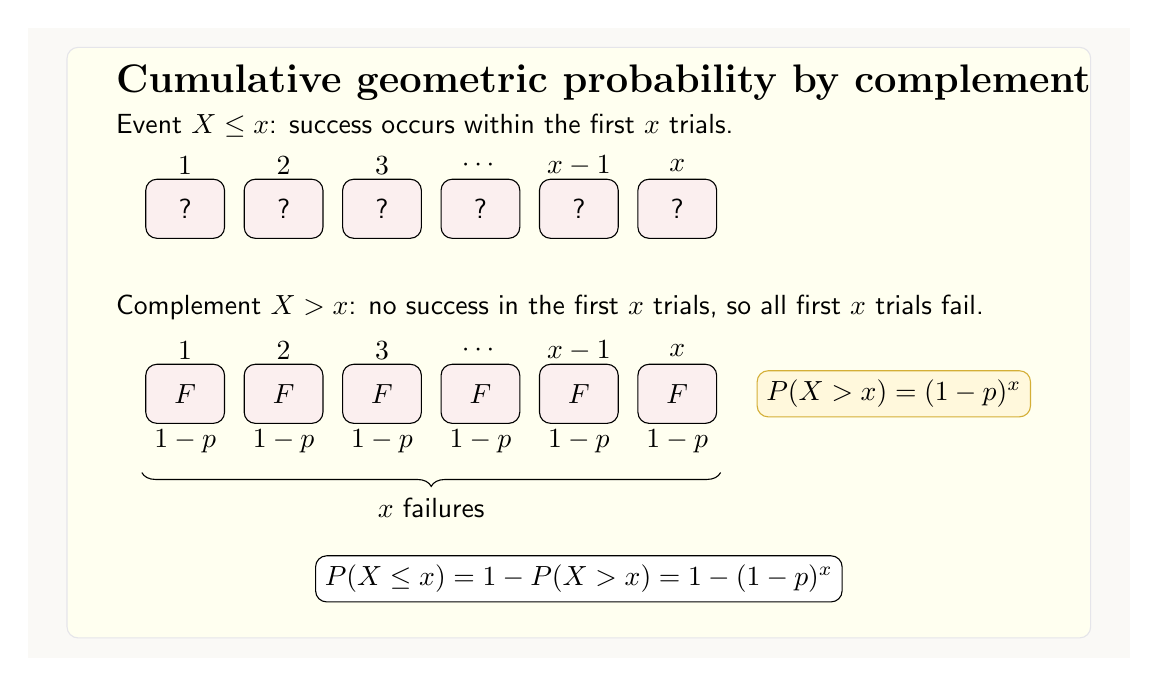
\begin{tikzpicture}[font=\sffamily]
\fill[fill={rgb,255:red,250;green,249;blue,246}] (-1,-5) rectangle (13,3);
\node[draw={rgb,255:red,229;green,229;blue,234},fill={rgb,255:red,255;green,255;blue,240},rounded corners,minimum width=13cm,minimum height=7.5cm] at (6, -1) {};
\node[anchor=west,font=\bfseries\Large] at (0,2.3) {Cumulative geometric probability by complement};
\node[anchor=west] at (0,1.75) {Event $X\le x$: success occurs within the first $x$ trials.};
\foreach \i/\lab in {0/1,1/2,2/3,3/\cdots,4/x-1,5/x}{\node[draw,rounded corners,fill={rgb,255:red,251;green,239;blue,239},minimum width=1cm,minimum height=.75cm] at (1+\i*1.25,.7) {?};\node at (1+\i*1.25,1.25) {$\lab$};}
\node[anchor=west] at (0,-.55) {Complement $X>x$: no success in the first $x$ trials, so all first $x$ trials fail.};
\foreach \i/\lab in {0/1,1/2,2/3,3/\cdots,4/x-1,5/x}{\node[draw,rounded corners,fill={rgb,255:red,251;green,239;blue,239},minimum width=1cm,minimum height=.75cm] at (1+\i*1.25,-1.65) {$F$};\node at (1+\i*1.25,-1.1) {$\lab$};\node at (1+\i*1.25,-2.25) {$1-p$};}
\draw[decorate,decoration={brace,mirror,amplitude=5pt}] (.45,-2.65)--(7.8,-2.65) node[midway,yshift=-.45cm] {$x$ failures};
\node[draw={rgb,255:red,212;green,175;blue,55},fill={rgb,255:red,255;green,248;blue,220},rounded corners,align=center] at (10,-1.65) {$P(X>x)=(1-p)^x$};
\node[draw,fill=white,rounded corners] at (6,-4) {$P(X\le x)=1-P(X>x)=1-(1-p)^x$};
\end{tikzpicture}
\end{document}
